\documentclass{article}
\usepackage[letterpaper, margin=1in]{geometry}
\usepackage{fixltx2e}
\usepackage{listings}
\usepackage{graphicx} % Required for inserting images
\usepackage{setspace}
\usepackage{multirow}
\usepackage{float}
\usepackage[sorting=none]{biblatex}
\addbibresource{labreport.bib}

\setstretch{1.50}
\title{
\textbf{Laboratory Report} \\
\huge Distributing parts of a Matrix over Sockets\\
\large CMSC 180: Introduction to Parallel Computing
}
\author{Jasrel Roby Peralta}
\date{May 2023}

\sloppy
\begin{document}

\maketitle

\section*{Introduction}
\hspace{\parindent} By using the serial computer program to interpolate a \emph{n x n} matrix, use \emph{t} number of slaves to interpolate \emph{n/t x n} submatrices using an open socket. Compare and analyze the runtimes when using a single machine and different machines.

\section*{Objectives}
The goal for this exercise is the following:
\begin{itemize}
    \item compare the running time of distributing \emph{n/t x n} submatrices in a single machine and distributing \emph{n/t x n} submatrices in different machines.
    \item determine if the implementation of the distribution of submatrices is efficient or not.
    \item determine which basic communication technique was employed in the implementation of the distribution of submatrices.
\end{itemize}

\section*{Methodology}
\hspace{\parindent} The machine used for this exercise is running on Ubuntu 22.04.2 LTS x86\_64, Intel i-7 8700 (12 cores) @ 4.60GHz, AMD ATI Radeon HD 8570 / RS 430, with 16GB memory. The programming language used in the computer program is Python 3.10.6. The interpolating algorithm used was the Federal Communications Commission (FCC) method. The graphing software used for making the charts is LibreOffice Calc. \\
\indent The computer program starts by asking the user what kind of instance is being run. The user may choose to input for the instance to be the \emph{master} or to be the \emph{slave}. The \emph{master} instance creates a random \emph{n x n} matrix, and starts a socket that listens on the port that is listed in the configuration file. It is also the duty of the \emph{master} to divide the matrix into \emph{t} equal parts, where \emph{t} is the number of \emph{slaves} to connect, which can also be found in the configuration file. If the experiment is done using different machines, the IP address of the \emph{master} instance is also needed, which is also found in the configuration file. The \emph{slave} instance connects and receives the matrix, then sends an acknowledgement to the \emph{master} that they have received the matrix and the columns they are set to interpolate. \\
\indent For each \emph{master-slave} connection, a thread is created. The program made use of the \emph{multithreading} module of Python 3.10.6. The timer starts when a created thread starts sending the data to another \emph{slave} instance. The timer ends when all the acknowledgements are received. For each run, \emph{n x n} matrix and t number of slaves are used. The three (3) runtimes are averaged and recorded to a table. The experiment is repeated for different values of \emph{n} and \emph{t}.\\


\section*{Results and Discussion}
\hspace{\parindent} After running the code three (3) successive times for each \emph{n x n} matrix size and \emph{t} slaves in a single machine, the following table is produced:

\begin{table}[H]
    \centering
    \noindent\makebox[\textwidth]{
    \begin{tabular}{|c|c|ccc|c|}
    \hline
    \multirow{2}{*}{\textbf{\begin{tabular}[c]{@{}c@{}}n\\ (size of matrix)\end{tabular}}} & \multirow{2}{*}{\textbf{\begin{tabular}[c]{@{}c@{}}t\\ (number of slaves)\end{tabular}}} & \multicolumn{3}{c|}{\textbf{time elapsed}}                                                 & \multirow{2}{*}{\textbf{\begin{tabular}[c]{@{}c@{}}average runtimes\\ (in seconds)\end{tabular}}} \\ \cline{3-5}
                                                                                            &                                                                                          & \multicolumn{1}{c|}{\textbf{run 1}} & \multicolumn{1}{c|}{\textbf{run 2}} & \textbf{run 3} &                                                                                                   \\ \hline
    1000                                                                                   & 2                                                                                        & \multicolumn{1}{c|}{0.546964}       & \multicolumn{1}{c|}{0.426787}       & 0.451198       & 0.474983                                                                                          \\ \hline
    1000                                                                                   & 4                                                                                        & \multicolumn{1}{c|}{7.68691}        & \multicolumn{1}{c|}{6.381048}       & 3.465593       & 5.844517                                                                                          \\ \hline
    1000                                                                                   & 8                                                                                        & \multicolumn{1}{c|}{13.918114}      & \multicolumn{1}{c|}{13.540195}      & 17.092937      & 14.85041533                                                                                       \\ \hline
    1000                                                                                   & 16                                                                                       & \multicolumn{1}{c|}{33.997901}      & \multicolumn{1}{c|}{28.528515}      & 33.216317      & 31.91424433                                                                                       \\ \hline
    4000                                                                                   & 2                                                                                        & \multicolumn{1}{c|}{0.503187}       & \multicolumn{1}{c|}{0.559047}       & 0.606459       & 0.556231                                                                                          \\ \hline
    4000                                                                                   & 4                                                                                        & \multicolumn{1}{c|}{6.70034}        & \multicolumn{1}{c|}{5.622571}       & 5.158803       & 5.827238                                                                                          \\ \hline
    4000                                                                                   & 8                                                                                        & \multicolumn{1}{c|}{15.856215}      & \multicolumn{1}{c|}{12.655223}      & 14.039135      & 14.18352433                                                                                       \\ \hline
    4000                                                                                   & 16                                                                                       & \multicolumn{1}{c|}{36.258801}      & \multicolumn{1}{c|}{33.189858}      & 33.621938      & 34.35686567                                                                                       \\ \hline
    8000                                                                                   & 2                                                                                        & \multicolumn{1}{c|}{0.986576}       & \multicolumn{1}{c|}{1.009564}       & 0.987448       & 0.9945293333                                                                                      \\ \hline
    8000                                                                                   & 4                                                                                        & \multicolumn{1}{c|}{5.468988}       & \multicolumn{1}{c|}{7.02219}        & 6.028941       & 6.173373                                                                                          \\ \hline
    8000                                                                                   & 8                                                                                        & \multicolumn{1}{c|}{14.665985}      & \multicolumn{1}{c|}{25.566632}      & 13.577927      & 17.936848                                                                                         \\ \hline
    8000                                                                                   & 16                                                                                       & \multicolumn{1}{c|}{38.402711}      & \multicolumn{1}{c|}{41.006283}      & 38.447953      & 39.285649                                                                                         \\ \hline
    \end{tabular}}
    \caption{\label{table}Average runtimes of the program using a single machine, using different terminals}
    \end{table}          
    
\indent To further understand the table, the following line chart is created using LibreOffice:
\begin{figure}[H]
    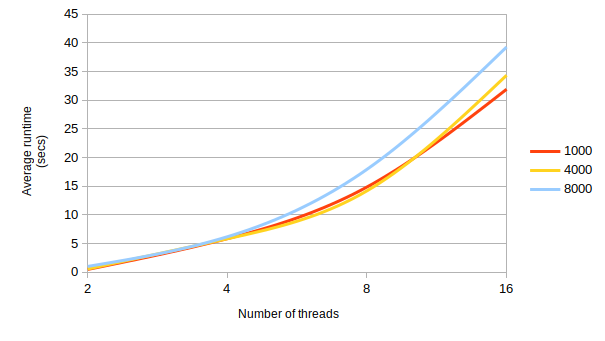
\includegraphics[width=0.8\textwidth]{chart01.png}
    \centering
    \caption{Line Chart of the Average runtimes of the program using a single machine, using different terminals}
    \end{figure}


\indent As seen from Table 1, the average running times for each \emph{n}-sized matrix increases as the \emph{t} number of slaves increases. The distribution of submatrices among two (2) \emph{slaves} finishes in \textless1 second, while distribution of submatrices among sixteen (16) slaves takes about \(\sim\)30 seconds. Though the average running time increases with the size of the matrix as well, the jump on average runtimes between each increase in the number of \emph{slaves} is more noticeable. \\
\indent The reason behind the significant jumps is the speed of the user running the program. Each \emph{slave} instance is needed to be ran manually, and while the earliest thread is already starting to send the data to a \emph{slave} instance, other \emph{slaves} are still being connected to the \emph{master}. Hence, connecting sixteen (16) \emph{slaves} takes up a large amount of time compared to connecting two (2) \emph{slaves}. \\

On the other hand, when running the program using different machines, the following table is produced:
\begin{table}[H]
    \centering
    \noindent\makebox[\textwidth]{
    \begin{tabular}{|c|c|ccc|c|}
    \hline
    \multirow{2}{*}{\textbf{\begin{tabular}[c]{@{}c@{}}n\\ (size of matrix)\end{tabular}}} & \multirow{2}{*}{\textbf{\begin{tabular}[c]{@{}c@{}}t\\ (number of slaves)\end{tabular}}} & \multicolumn{3}{c|}{\textbf{time elapsed}}                                                 & \multirow{2}{*}{\textbf{\begin{tabular}[c]{@{}c@{}}average runtimes\\ (in seconds)\end{tabular}}} \\ \cline{3-5}
                                                                                               &                                                                                          & \multicolumn{1}{c|}{\textbf{run 1}} & \multicolumn{1}{c|}{\textbf{run 2}} & \textbf{run 3} &                                                                                                   \\ \hline
    1000                        & 2                           & \multicolumn{1}{c|}{2.381978}       & \multicolumn{1}{c|}{1.258513}       & 1.362663       & 1.667718                          \\ \hline
    1000                        & 4                           & \multicolumn{1}{c|}{4.682795}       & \multicolumn{1}{c|}{2.638427}       & 5.022053       & 4.114425                          \\ \hline
    4000                        & 2                           & \multicolumn{1}{c|}{16.474031}      & \multicolumn{1}{c|}{12.706133}      & 17.209705      & 15.46328967                       \\ \hline
    4000                        & 4                           & \multicolumn{1}{c|}{31.801009}      & \multicolumn{1}{c|}{23.391966}      & 31.282571      & 28.825182                         \\ \hline
    8000                        & 2                           & \multicolumn{1}{c|}{46.978968}      & \multicolumn{1}{c|}{45.075998}      & 51.603052      & 47.886006                         \\ \hline
    8000                        & 4                           & \multicolumn{1}{c|}{119.868819}     & \multicolumn{1}{c|}{122.850237}     & 125.255857     & 122.6583043                       \\ \hline
    \end{tabular}}
    \caption{\label{table}Average runtimes of the program using different machines}
    \end{table}

\indent To further understand the table, the following line chart is created using LibreOffice:
\begin{figure}[H]
    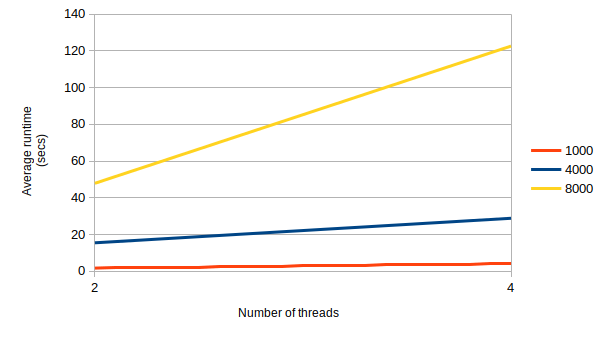
\includegraphics[width=0.8\textwidth]{chart02.png}
    \centering
    \caption{Line Chart of the Average runtimes of the program using different machines}}
    \end{figure}


\indent In Table 2, it is observed that the distribution time of the \emph{n/t x n} submatrices increases as the size of the matrix increases. Compared to Table 1 where the average running time heavily relied on the number of \emph{slaves}, the average running time in Table 2 relies on the size of the matrix. \\
\indent The reason for this is the time it takes for the matrix to be sent through the socket, and since the setup for Table 2 uses different machines, it took a lot more time distributing submatrices compared to distributing in a single machine. Also, large chunks of data are being sent. Hence, the bigger the amount of data needed to be sent to the \emph{slave}, the longer the time it takes to finish and send an acknowledgement to the \emph{master}.
    

\section*{Conclusion}
\hspace{\parindent} The distribution time of \emph{n/t x n} submatrices in a single machine is heavily dependent on the number of \emph{slaves} due to user factors, and the distribution time of \emph{n/t x n} submatrices in different machines is heavily dependent on the size of the matrix being interpolated. However, if the extra time it takes the user to manually connect other \emph{slaves} to the \emph{master}, the time is expected to drop significantly. This can be said due to the average running time of \emph{n}-sized matrices with two (2) \emph{slaves}. \\
\indent Moreover, the implementation of the distribution of is not efficient because it did not employ any basic communication techniques that was discussed in the lecture component. Also, the use of \emph{multiprocessing} Python module is a recommendation because the \emph{multithreading} Python module has a Global Interpreter Lock (GIL) which hinders the threads to run concurrently \cite{intro,gil,thread-based,multiprocessing}.


\printbibliography{}


\pagebreak
\section*{\centering Appendix}
\begin{center}
Main file for master-slave and interpolation \\ (main.py)
\end{center}
\setstretch{1}
\begin{lstlisting}[language=Python]
    import numpy as np
    import random
    import datetime
    import help
    import socket
    import threading
    import queue

    # global counter of received acknowledgements
    COUNTER_ACK = 0

    # prettier printing options
    np.set_printoptions(linewidth=1000, formatter={'float': '{: 0.0f}'.format})

    # get size of nxn matrix
    def getSize():
        n = 1
        while (n % 10 != 0):
            n = int(input("enter size of matrix: "))
            if n % 10 != 0:
                print('invalid size of matrix')
        return n+1

    # get port number
    def getPort():
        p = 0
        while (p < 5000) or (p > 65535):
            p = int(input('enter port number: '))
            if (p < 5000) or (p > 65535):
                print('invalid port number')
        return p

    # get status of the instance
    # 0 = master
    # 1 = slave
    def getInstance():
        s = 2
        while (s != 0) and (s != 1):
            s = int(input('enter status of instance: '))
            if (s != 0) and (s != 1):
                print('invalid status of instance')
        return s


    # interpolate function
    def terrain_inter(mat,x1,x2):
        for i in range(0,n):
            for j in range(x1,x2):
                if mat[i][j] != 0:
                    continue
                if (i % dist == 0):
                    get_row_val(i,j)
        for i in range(0,n):
            for j in range(x1,x2):
                if (mat[i][j] == 0):
                    get_col_val(i,j)

    def get_nearest_row(i,j,dir):
        # go up
        if dir < 0:
            dir = j - (j % 10)
        # go down
        else:
            dir = j + (10 - (j % 10))
        return [dir,mat[i][dir]]

    def get_nearest_col(i,j,dir):
        # go left
        if dir < 0:
            dir = i - (i % 10)
        # go right
        else:
            dir = i + (10 - (i % 10))
        return [dir,mat[dir][j]]

    # follow given FCC formula
    def fcc(x1,y1,x2,y2,x):
        return (y1 + (((x-x1)/(x2-x1)) * (y2-y1)))

    # interpolate rows with random values
    def get_row_val(i,j):
        dp = get_datapoints_row(i,j)
        x = j               # j -> row
        x1 = dp[0][0]
        x2 = dp[1][0]
        y1 = dp[0][1]
        y2 = dp[1][1]
        res = fcc(x1,y1,x2,y2,x)
        mat[i][j] = res

    # interpolate columns
    def get_col_val(i,j):
        dp = get_datapoints_col(i,j)
        # dp = [[x1,y1][x2,y2]]
        x = i               # i -> col
        x1 = dp[0][0]
        x2 = dp[1][0]
        y1 = dp[0][1]
        y2 = dp[1][1]
        res = fcc(x1,y1,x2,y2,x)
        mat[i][j] = res


    def createMatrix(n, dist):
        # create a zero nxn matrix
        mat = np.zeros((n,n), dtype = float)

        # randomize elevation values for gridpoints divisible by 10
        for i in range(n):
            for j in range(n):
                if i % dist == 0 and j % dist == 0:
                    mat[i][j] = random.uniform(0.0, 1000.0)
            
        return mat


    # get closest datapoints to the current gridpoint
    def get_datapoints_row(i,j):
        dp = []
        dp.append(get_nearest_row(i,j,-1))
        dp.append(get_nearest_row(i,j,+1))
        return dp
    def get_datapoints_col(i,j):
        dp = []
        dp.append(get_nearest_col(i,j,-1))
        dp.append(get_nearest_col(i,j,+1))
        return dp

    # convert matrix to string
    def matToString(mat):
        mat = mat.tobytes()
        return mat

    # convert string to matrix
    def stringToMat(data):
        mat = np.frombuffer(data)
        mat = np.reshape(mat, (n,n))
        return mat

    # send and receive data from slave for each thread
    def sendReceiveData(conn, mat, start, end, queue):
        # send data to slave
        mat = matToString(mat)
        help.send_msg(conn, mat)

        # send start and end indices to slave
        indices = [start, end]
        indices = np.array(indices)
        indices = indices.tobytes()
        help.send_msg(conn, indices)

        if conn.recv(1024) == b'ack':
            global COUNTER_ACK
            COUNTER_ACK += 1
            print('acknowledgement received from', conn.getpeername())


        # receive data from slave
        data = help.recv_msg(conn)
        data = stringToMat(data)

        # update matrix
        mat = data

        # close connection
        conn.close()

        # return updated matrix
        queue.put(mat)

    # divide matrix into t parts to be sent to t threads
    def divideMatrix(mat, t):
        # get size of matrix
        n = mat.shape[0]

        # get number of rows per thread
        rows = n // t

        # get start and end indices for each thread
        # if n is divisible by t
        if n % t == 0:
            start = 0
            end = rows
            indices = []
            for i in range(t):
                indices.append([start, end])
                start = end
                end += rows
        else:
            start = 0
            end = rows + (n % t)
            indices = []
            for i in range(t):
                indices.append([start, end])
                start = end
                end += rows

        # return indices
        return indices

    # update matrix with data from slave
    def updateMatrix(mat, data):
        # update matrix
        for i in range(n):
            for j in range(n):
                if mat[i][j] == 0:
                    mat[i][j] = data[i][j]

        # return updated matrix
        return mat

    # main function
    if __name__ == "__main__":
        # initialize data
        n = getSize()
        s = getInstance()

        # initialize distance between gridpoints
        dist = 10

        # master instance
        if s == 0:
            # create matrix
            mat = createMatrix(n, dist)

            # print matrix
            print(mat)

            # read config file
            f = open('config.in', 'r')
            lines = f.readlines()
            f.close()

            # get number of slaves, ip address, and port number
            num_slaves = int(lines[0])
            ip_address = lines[1].strip('\n')
            port = int(lines[2])

            # start server
            s = socket.socket(socket.AF_INET, socket.SOCK_STREAM)
            

            # counter for number of slaves connected
            counter = 0
            with s:
                # bind socket to ip address and port
                s.bind((ip_address, port))
                print('server started on port', port)
                
                # start listening
                s.listen(num_slaves)
                print('server started listening on port', port)
                
                # list of threads
                threads = []

                # divide matrix into t parts
                indices = divideMatrix(mat, num_slaves)
                
                # create queue to store results
                q = queue.Queue()
                counter_again = 0

                while True and (COUNTER_ACK != num_slaves):
                    # accept connections
                    conn, addr = s.accept()
                    print('connected to', addr)

                    #start timer
                    if counter_again == 0:
                        print('start timer')
                        start = datetime.datetime.now()
                        counter_again = 1

                    # create thread
                    thread = threading.Thread(target = sendReceiveData, args = (conn, mat, indices[counter-1][0], indices[counter-1][1], q))
                    threads.append(thread)
                    thread.start()
                    print("thread", counter, "started running")
                    counter += 1
                    
                    if counter == num_slaves:
                        break
                
                # keep looping until all acknowledges are received
                while COUNTER_ACK != num_slaves:
                    continue

                # stop timer since all slaves are connected
                end = datetime.datetime.now()
                print('time elapsed during distributing:', end-start)
                
                # wait for all threads to finish then update matrix
                print('waiting for threads to finish...')
                for thread in threads:
                    thread.join()
                    mat = updateMatrix(mat, q.get())
                        

            # print matrix
            print(mat)

            # stop server
            s.close()

            # stop another timer
            end = datetime.datetime.now()
            print('time elapsed w/ interpolation:', end-start)

            # print message
            print('server stopped listening on port', port)
            print('server closed')
            




        # slave instance
        else:
            # read config file
            f = open('config.in', 'r')
            lines = f.readlines()
            f.close()

            # get number of slaves, ip address, and port number
            num_slaves = int(lines[0])-1
            ip_address = lines[1].strip('\n')
            port = int(lines[2])

            # connect to master
            s = socket.socket(socket.AF_INET, socket.SOCK_STREAM)
            s.connect((ip_address, port))


            
            # receive matrix from master
            mat = help.recv_msg(s)
            mat = stringToMat(mat)



            # get start and end indices for slave
            indices = help.recv_msg(s)
            indices = np.frombuffer(indices, int)
            indices = np.reshape(indices, (2,1))
            start = int(indices[0])
            end = int(indices[1])

            # send acknowledgement to master
            s.sendall(b'ack')


            # interpolate matrix
            print("interpolating from ", start, " to ", end)
            terrain_inter(mat, start, end)
            print(mat)

            # send matrix back to master
            mat = matToString(mat)
            help.send_msg(s, mat)
            s.close()


\end{lstlisting}
\pagebreak
\begin{center}
    Helper file for handling connections \\ (help.py)
\end{center}
\setstretch{1}
\begin{lstlisting}[language=Python]
    import struct
    import itertools
    import threading
    import time
    import sys

    #here is the animation
    def animate(done):
        for c in itertools.cycle(['|', '/', '-', '\\']):
            if done:
                break
            sys.stdout.write('\rloading ' + c)
            sys.stdout.flush()
            time.sleep(0.1)
        sys.stdout.write('\rDone!     ')


    def start(do_this, *args):
        done = False
        t = threading.Thread(target=animate, args=(done))
        t.start()

        
        x = threading.Thread(target=do_this, args=(args))
        x.start()
        x.join()

        done = True
        t.join()


    def send_msg(sock, msg):
        # Prefix each message with a 4-byte length (network byte order)
        msg = struct.pack('>I', len(msg)) + msg
        sock.sendall(msg)

    def recv_msg(sock):
        # Read message length and unpack it into an integer
        raw_msglen = recvall(sock, 4)
        if not raw_msglen:
            return None
        msglen = struct.unpack('>I', raw_msglen)[0]
        # Read the message data
        return recvall(sock, msglen)

    def recvall(sock, n):
        # Helper function to recv n bytes or return None if EOF is hit
        data = bytearray()
        while len(data) < n:
            packet = sock.recv(n - len(data))
            if not packet:
                return None
            data.extend(packet)
        return data
\end{lstlisting}
\end{document}
